    %CPU y GPU -> femeninos
    %Schedule -> planificación
    %Preemptive -> preventivo
    %Preemption -> prevención
    %----------------------------------------------------------------------
    %RESUMEN
    El objetivo de este capítulo es introducir los conceptos de: 
    \begin{inparaenum}
    \item Framework;
    \item Sistemas en tiempo real;
    \item Tipos de ejecución de tareas; 
    \item El algoritmo por defecto de los sistemas en tiempo real; 
    \item Sstemas embebidos heterogéneos; 
    \item Arquitecturas de hardware y software de tarjetas gráficas; y 
    \item Cómputo de propósito general en unidades de procesamiento de gráficos.
    \end{inparaenum}
    %----------------------------------------------------------------------
     %INGENIERIA DE SOFTWARE
     \section{Ingeniería de Software}

 El Instituto de Ingeniería Eléctrica y Electrónica (Institute of Electrical and Electronics Engineers – IEEE) define a la Ingeniería de Software como:

\begin{quote}
\textit{"La Ingeniería de Software\cite{IeeeSG} es la aplicación de un enfoque sistemático, disciplinado y cuantificable al desarrollo, operación y mantenimiento de software; es decir, la aplicación de la ingeniería al software."}
\end{quote}

La Ingeniería de Software aplica diferentes técnicas, normas y métodos que permiten obtener mejores resultados al desarrollar y usar piezas software, al tratar con muchas de las áreas de Ciencias de la Computación es posible llegar a cumplir de manera satisfactoria con los objetivos fundamentales de la Ingeniería de Software. Entre los objetivos de la Ingeniería de Software están\cite{enSWE}:

\begin{itemize}
\item Mejorar el diseño de aplicaciones o software de tal modo que se adapten de mejor manera a las necesidades de las organizaciones o finalidades para las cuales fueron creadas.
\item Promover mayor calidad al desarrollar aplicaciones complejas.
\item Brindar mayor exactitud en los costos de proyectos y tiempo de desarrollo de los mismos.
\item Aumentar la eficiencia de los sistemas al introducir procesos que permitan medir mediante normas específicas la calidad del software desarrollado, buscando siempre la mejor calidad posible según las necesidades y resultados que se quieren generar.
\item Una mejor organización de equipos de trabajo, en el área de desarrollo y mantenimiento de software.
\item Detectar a través de pruebas, posibles mejoras para un mejor funcionamiento del software desarrollado     
\end{itemize}     
     
     \subsection{Framework}
Un framework o marco de trabajo es la estructura que se establece para normalizar, controlar y organizar, ya sea, una aplicación completa, o bien, una parte de ella. Esto representa una ventaja para los participantes en el desarrollo del sistema, ya que automatiza procesos y funciones habituales, además agiliza la codificación de ciertos mecanismo ya implementados al reutilizar código.
Un framework puede ser considerada como un molde configurable, al que podemos añadirle atributos especiales para finalmente construir una solución completa.

\vspace{0.3cm}
La utilización de un framework siempre conlleva una curva de de aprendizaje, pero a largo plazo facilita la programación, escalabilidad, y el mantenimiento de los sistemas.
		
    %SISTEMAS EN TIEMPO REAL
    \section{Sistemas en tiempo real}\label{sec:sistr}

    Los sistemas en tiempo real son sistemas de cómputo cuyas tareas deben actuar dentro de limitaciones de tiempo precisas ante eventos en su entorno. Por lo que el comportamiento del sistema depende, no solo del resultado del cálculo, sino también del momento (tiempo) en qué se produce \cite{Buta2011}.
    
    Un sistema en tiempo real debe  responder a entradas generadas dentro de un periodo de tiempo especifico para evitar posibles fallas. El deadline o tiempo límite es el momento justo antes en que la tarea debe completar su ejecución. Existen tres tipos de plazos: 
%time constrains: plazos de tiempo
%deadline: tiempo limite
\begin{itemize}
\item Soft Deadline: En este tipo se pueden superar algunos tiempos límites y el sistema puede aún funcionar correctamente.
\item Firm Deadline: Aquí los resultados obtenidos en los plazos vencidos no son útiles, pero los plazos son tolerados frecuentemente.
\item Hard Deadline: Si una tarea no se cumple en el tiempo límite, se producirán resultados catastróficos. Este tipo de límites se utilizan comúnmente en tareas que realizan operaciones críticas.
\end{itemize}   

\subsection{Tipos de tarea}

Existen tres tipos de tareas que están presentes en los sistemas en tiempo real:

\begin{itemize}
\item Tareas periódicas: Se ejecutan en cada intervalo fijo de tiempo conocido. Normalmente, las tareas periódicas tienen restricciones que indican sus plazos de tiempo.
\item Tareas aperiódicas: Se ejecutan aleatoriamente en cualquier plazo de tiempo y no tienen una secuencia de tiempo predefinida.
\item Tareas esporádicas: Son una combinación de tareas periódicas y aperiódicas, donde, en tiempo de ejecución actúan como aperiódicas pero la tasa de ejecución es de naturaleza periódica.
\end{itemize}   

La mayoría del tiempo los plazos de tiempo se dan por el tiempo límite de una tarea.

    \subsection{Esquemas de planificación}
    
        \subsubsection{Planificación cooperativa}

En en el esquema de planificación \textit{\textbf{cooperativa}} o non-preemptive las tareas deciden el tiempo que utilizarán los recursos de cómputo, el trabajo del planificador es únicamente el de asignar tareas a los nodos de procesamiento disponibles.      

  \begin{figure}[ht]
      \centering
        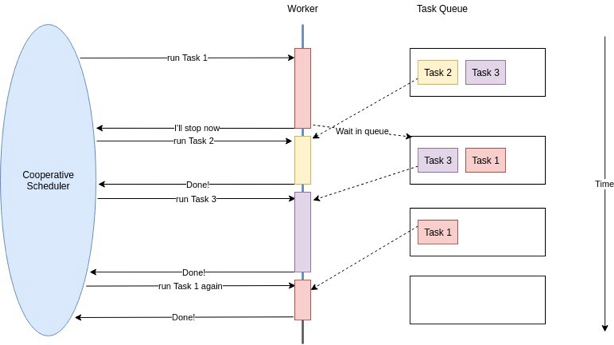
\includegraphics[scale=1.5]{img/schedCoo}
        \caption{Planificación cooperativa.\cite{medium}}
        \label{fig:schedcoo}
    \end{figure}
    
El problema de esto es que una tarea puede absorber todos los recursos del sistema generando plazos vencidos en las demás tareas.

  \begin{figure}[ht]
      \centering
        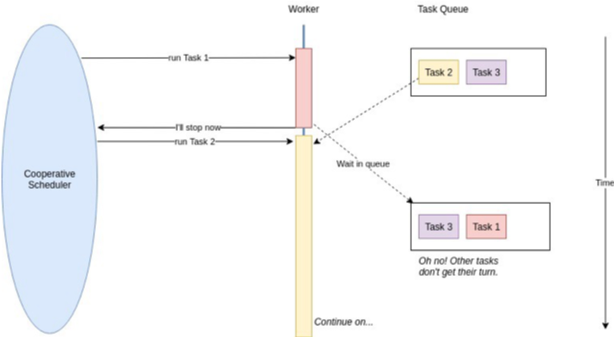
\includegraphics[scale=1.5]{img/schedCooDead}
        \caption{Planificación cooperativa con plazos vencidos.\cite{medium}}
        \label{fig:schedcoodead}
    \end{figure}
    
\subsubsection{Planificación preemptive}

En este esquema, el planificador es el que tiene la batuta ante las tareas, las asigna a los recursos disponibles, y les define un tiempo de ejecución máximo, comúnmente llamado quantum\cite{PreeK}. Superado este punto, el planificador interrumpe (preempts) la tarea para que otra sea ejecutada en su lugar, y la tarea interrumpida debe esperar hasta que le toque su turno nuevamente.

  \begin{figure}[ht]
      \centering
        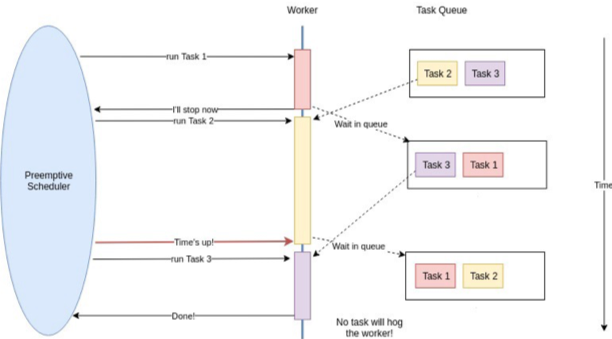
\includegraphics[scale=1.5]{img/schedPre}
        \caption{Planificación preemptive.\cite{medium}}
        \label{fig:schedpree}
    \end{figure}
    
    

Debido a que muchas veces se interrumpen tareas a la mitad de un proceso, es necesario almacenar y restaurar el estado que se tenia antes de dicha interrupción para continuar justo en el punto en donde se quedó.

A este proceso de almacenamiento, intercambio y restauración del estado de las tareas se le denomina \textbf{cambio de contexto} (\textbf{context switch}).

    \subsection{Algoritmos de planificación}\label{sec:AlgoPlan}. 
    
    Un algoritmo de planificación es una estrategia en la cual un sistema decide ejecutar una tarea en un momento dado, debe garantizar que se asigne el tiempo suficiente a todas las tareas del sistema para que puedan cumplir su tiempo límite en la medida de lo posible.
    
    La planificación en tiempo real se puede dividir en:
    \begin{itemize}
    \item Estática:  todas las prioridades se asignan en el momento del diseño del sistema y esas prioridades se mantienen constantes durante el tiempo de vida de una tarea.
    \item Dinámica: Se las asignan prioridades en tiempo de ejecución, en función de los parámetros de las tareas. Su objetivo es adaptarse al progreso del sistema para buscar la configuración óptima de planificación.
    \end{itemize}   

        \begin{table}[h!]
      \begin{center}
            \scriptsize
        \begin{tabular}{|m{1.5cm}|m{2cm}|m{2cm}|m{2cm}|m{2cm}|m{3cm}|}
         \hline
        \cellcolor{lightgray}\textbf{Algoritmo} & \cellcolor{lightgray} \textbf{Asignación de prioridad} & \cellcolor{lightgray} \textbf{Criterio de planificación} & \cellcolor{lightgray} \textbf{Preemptive/ Non-preemptive} & \cellcolor{lightgray} \textbf{Utilización de CPU} & \cellcolor{lightgray} \textbf{Eficiencia}  \\ 
         \hline
          \textbf{SJF} & Estática & Tiempo de Ejecución & Non-preemptive & 100\% & Eficiente con tareas de finalización oportuna \\
         \hline
         \textbf{EDF} & Dinámica & Plazo Límite & Preemptive & 100\% & Eficiente en condiciones subcargadas \\
         \hline 
         \textbf{RM} & Estática & Periodo & Preemptive & < 100\% & Eficiente en condiciones sobrecargadas \\
         \hline
          \textbf{DM} & Estática & Plazo Límite Relativo & Preemptive & > a RM & Eficiente \\
         \hline
          \textbf{LLF} & Dinámica & Laxitud & Preemptive & 100\% & Eficiente \\
         \hline
          \textbf{GEDF} & Dinámica & Plazo Límite y Tiempo de ejecución & Non-preemptive & 100\%& Eficiente en ambientes Non-preemptive \\
         \hline
                \end{tabular}
        \caption{Matriz de comparación de algoritmos de planificación.}
        \label{tab:table2}
      \end{center}
    \end{table}
    
    \subsubsection{Shortest Job First}
    Shortest Job First (SJF) es el algoritmo de planificación que asigna la prioridad mayor a la tarea con el menor tiempo de ejecución. SJF es el algoritmo más utilizado cuando se comienzan a estudiar los sistemas en tiempo real debido a su simplicidad y porque minimiza la cantidad promedio de tiempo que cada tarea debe esperar hasta que se complete su ejecución \cite{Tanenbaum}. Este algoritmo funciona únicamente con tareas non-preemptive, por lo que fácilmente puede llegarse a un estado de inanición de tareas que requieren mucho tiempo para completarse si se agregan continuamente tareas pequeñas.
    
    \subsubsection{Earliest Deadline First} 
    Earliest Deadline First (EDF) es un algoritmo con prioridad dinámica, en el que la tarea con el plazo fijo más próximo tiene la máxima prioridad. Este algoritmo es óptimo para implementación sobre un único procesador, y cuando el sistema se encuentra en bajos y moderados niveles de contención de recursos y datos\cite{Liu}. Ya que cuando se sobrecarga el sistema, la mayoría de las tareas obtienen una alta prioridad, lo que termina en un rendimiento disminuido.
    
     \vspace{0.3cm}
     
    Es un algoritmo muy extendido en sistemas en tiempo real debido a su optimalidad teórica en el campo no-preemptive, pero al momento de implementarlo en un planificador preemptive, el resultado puede acarrear un exceso de ejecución si se toma el peor caso \cite{EmbSysDes}. Por ello es necesario buscar alternativas de algoritmos que tengan un mejor desempeño en tareas específicas.
    
     \subsubsection{Rate Monotonic}
    Rate Monotonic (RM) es un algoritmo de planificación preemptive con prioridad estática para un solo procesador\cite{Liu}. RM asigna la prioridad más alta a la tarea con el periodo más corto, suponiendo que los periodos sean igual a los plazos \( (P_{i} = D_{i}) \), esto porque si la tasa de demanda es mayor, el periodo sería más corto y por ende, la prioridad aumentaría. Por ello es optimo para usarse en tareas periódicas. La mayor limitación de su implementación, es que al utilizar tareas de prioridad fija no siempre se utiliza el 100\%  del CPU, lo que conlleva al posible desperdicio de recursos\cite{RM}.

\subsubsection{Deadline Monotonic}
Deadline Monotonic (DM) es el algoritmo óptimo de planificación con prioridad fija donde las prioridades son asignadas inversamente proporcionales a los plazos fijos, con esto cuando se cumple que el plazo es menor al tiempo de la tarea (D < T) cuando el periodo es igual que el plazo limite (P = D) podemos ver a RM como un caso especial de DM \cite{NPr}. DM ejecuta en cada instante de tiempo la tarea con el plazo más corto, por lo que si dos más tareas tienen el mismo plazo limite se debe elegir aleatoriamente la siguiente en ejecutarse.

\subsubsection{Least Laxity First}
Least Laxity First (LLF) es un algoritmo óptimo de planificación con prioridad dinámica. La laxitud de una tarea está definida como el plazo límite menos el tiempo de ejecución restante, está laxitud es la cantidad máxima de tiempo que un trabajo puede esperar cumpliendo su plazo límite. En este algoritmo, se otorga la máxima prioridad al trabajo con la menor laxitud, se permite que la tarea actualmente en ejecución sea intercambiada por otra con menor laxitud en cualquier momento \cite{NPr}.
  \vspace{0.3cm}
  
  El punto débil de este algoritmo se presenta cuando dos tareas presentan la misma laxitud, ya que un proceso se ejecutará durante un período corto de tiempo y luego será reemplazado por el otro y viceversa, obteniendo numerosos cambios de contexto durante la vida útil de las tareas mermando el rendimiento del sistema en general. Este algoritmo es óptimo para sistemas con tareas periódicas \cite{ComRTT}.

\subsubsection{Group Earliest Deadline First}
Group Earliest Deadline First (GEDF) está pensado para mejorar el desempeño de EDF durante condiciones de sobrecarga. La idea principal de su funcionamiento es agrupar las tareas con plazo límite similares y dentro de cada grupo planificar las tareas con SJF \cite{ComRTT}. El parámetro rango de grupo (Gr) determina qué tarea ingresa a qué grupo el cuál es un porcentaje de la tarea al comienzo del plazo absoluto de cada cola.

%Aunque existen protocolos más simples y fáciles de implementar, como lo es la planificación non-preemtive, pueden llegar a provocarse bloqueos en el sistema en tareas críticas de seguridad. 

    %----------------------------------------------------------------------
    %GPU
    \section{CPU}
    La unidad de procesamiento central o CPU es un procesador de propósito general, lo que significa que puede hacer una variedad de cálculos, pero esta diseñado para realizar el procesamiento de información en serie, consta de pocos núcleos de propósito general. Aunque se pueden utilizar bibliotecas para realizar concurrencia y paralelismo, el hardware \textit{per se} no tiene esa implementación.

     \subsection{Arquitectura del CPU}

Un CPU está compuesto principalmente por:
\begin{itemize}
\item Reloj: elemento que sincroniza las acciones del CPU.
\item ALU (Unidad lógica y aritmética): como su nombre lo indica, soporta pruebas lógicas y cálculos aritméticos, y puede procesar varias instrucciones a la vez.
\item Unidad de Control: se encarga de sincronizar los diversos componentes del procesador.
\item Registros: memorias de tamaño pequeño, del orden de bytes, y que son lo suficientemente rápidas para que el ALU manipule su contenido en cada ciclo de reloj.
\item Unidad de entrada-salida (I/O): soporta la comunicación con las memoria de la computadora y permite el acceso a los periféricos.
\end{itemize}   

    \section{GPU}
   
    La unidad de procesamiento gráfico o GPU es un procesador especializado para tareas que requieren de un alto grado de paralelismo. Su uso más extendido es el del procesamiento de instrucciones aplicadas a campo de imágenes 2D y 3D, realizando cálculos con pixeles y texeles\cite{TX2CU}.
    
   \vspace{0.3cm}
   
   La tarjeta gráfica en su interior puede contener una cantidad de núcleos de un orden de cientos hasta miles de unidades que son más pequeñas y que por ende, individualmente realizan un menor número de operaciones. Esto hace que la GPU esté optimizada para procesar cantidades enormes de datos pero con programas más específicos\cite{gpgpu}. Lo más común al utilizar la aceleración por GPU es ejecutar una misma instrucción a múltiples datos para aprovechar su arquitectura.
   
    \subsection{Arquitectura del GPU}

La arquitectura de las tarjetas gráficas ha ido experimentando ciertas evoluciones en su desarrollo para permitir a los programadores hacer un uso más eficiente de su poder de procesamiento. Contienen en su interior componentes no de cómputo no especializado para procesar todo tipo de información.

Una tarjeta gráfica es básicamente un multiprocesador compuesto de una gran cantidad de núcleos de procesamiento que trabajan en paralelo, junto con los componentes de un CPU, las GPU incorporan:

\begin{itemize}
\item Memoria: cuentan con diferentes tipos de memoria y principalente compuesta por el tipo DRAM (Memoria dinámica de acceso aleatorio).
	\begin{itemize}
	\item Memoria global: Almacena los datos enviados desde el CPU.
	\item Memoria constante de sólo lectura.
	\item Memoria de texturas de sólo lectura.
	\item Registros locales por núcleo de 32 bits. 
	\end{itemize}
Donde las memorias constantes y de textura son de acceso más rápidas que la memoria global, ya que actúan como una especie de caché.

\item Programación en streams: La arquitectura de una GPU está diseñada con base en la programación de streams, el cual involucra a múltiples cálculos en paralelo para un stream de datos\cite{stream}. 

	\begin{itemize}
	\item Stream: Conjunto de elementos que tendrán un tratamiento similar.
	\item Kernel: Tratamiento aplicado a cada elemento del stream.
	\item Thread: Tratamiento ejecutado por procesador aplicado a un elemento del stream.
	\end{itemize} 
	
\item Gather y Scatter: Cuando se aplica un kernel a un stream, este aplica todas sus instrucciones a cada elemento, por lo que cada elemento se almacena en un una posición bien definida dentro de la memoria utilizando indices que auxilian a localizarlo, a esta acción se le conoce como Scatter. 

        \begin{figure}[ht]
      \centering
        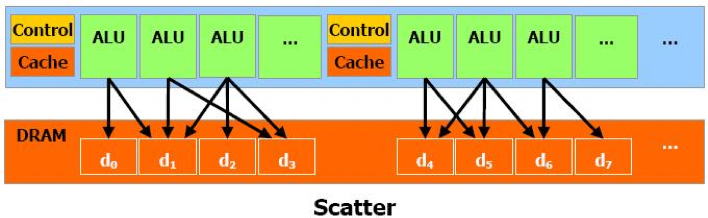
\includegraphics[scale=1]{img/scatter}
        \caption{Escritura en DRAM\cite{NCUDA}.}
        \label{fig:scatter}
    \end{figure}
   
En cambio el Gather es la lectura o recolección de un stream en memoria para ser procesado por una unidad de procesamiento.

        \begin{figure}[ht]
      \centering
        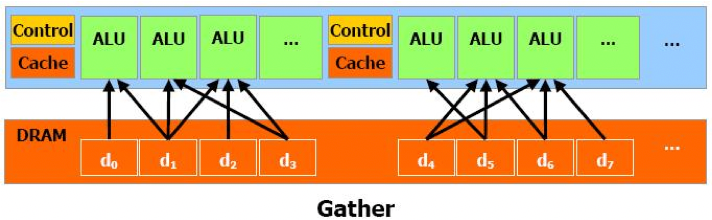
\includegraphics[scale=1]{img/gather}
        \caption{Lectura en DRAM\cite{NCUDA}.}
        \label{fig:gather}
    \end{figure}

\end{itemize} 
    \subsection{Manycore y Multicore}
    Es necesario destacar que los \textit{manycore} y los \textit{multicore} son utilizados para etiquetar a los CPU y los GPU, pero entre ellos existen diferencias. Un core de CPU es relativamente más potente, está diseñado para realizar un control lógico muy complejo para buscar y optimizar la ejecución secuencial de programas.
   
    \vspace{0.3cm}
    En cambio un core de GPU es más ligero y está optimizado para realizar tareas de paralelismo de datos como un control lógico simple enfocándose en la tasa de transferencia (\textit{throughput}) de los programas paralelos.
    
        \begin{figure}[ht]
      \centering
        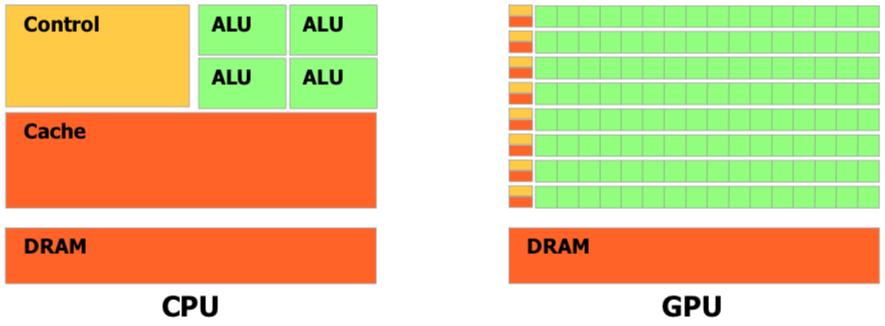
\includegraphics[scale=0.35]{img/repCPUGPU}
        \caption{Representación de un CPU y un GPU\cite{NCUDA}.}
        \label{fig:gpgpu}
    \end{figure}
    
    \vspace{0.3cm}
    Con aplicaciones computacionales intensivas, las secciones del programa a menudo muestran una gran cantidad de paralelismo de datos. Las GPU se usan para acelerar la ejecución de esta porción código. Cuando un componente de hardware que está físicamente separado de la CPU y se utiliza para acelerar secciones computacionalmente intensivas de una aplicación, se le denomina acelerador de hardware. Se puede decir que las GPU son el ejemplo más común de un acelerador de hardware.

    \subsection{Arquitectura Pascal}

    La principal ventaja de la arquitectura Pascal está en su construcción ya que está implementada con transistores FinFET\cite{PasGPU}, los cuales a ser de un tamaño de 16 nanometros, permiten tener un tamaño reducido, proporcionar un rendimiento alto y obtener una gran eficiencia energética. Dicha combinación la hacen ideal para ser implementada en dispositivos embebidos que requieran ejecutar tareas híbridas.
     
    \subsubsection{Memoria unificada} \label{sec:MemUni}
     La memoria unificada proporciona un único espacio de direcciones virtuales para la memoria de la CPU y GPU, permitiendo la migración transparente de datos entre los espacios de direcciones virtuales completos tanto de la tarjeta gráfica como del procesador. Esto simplifica la programación en GPUs y su portabilidad ya que no es necesario el  preocuparse por administrar el intercambio de datos entre dos sistemas de memoria virtual diferentes\cite{WPNV}.
     
    %Asignar memoria unificada es tan simple como reemplazar llamadas a malloc o cudaMalloc con llamadas a cudaMallocManaged\cite{}.
     
    \subsubsection{Computación preemptive}
    Permite que las tareas de cómputo se reemplacen con granularidad a nivel de instrucción, en lugar de bloque de subprocesos, evitando el funcionamiento prolongado de aplicaciones que monopolizan el sistema y no dejan ejecutar terceras tareas\cite{WPNV}. Obteniendo así, que las tareas puedan ejecutarse todo el tiempo que requieran ya sea para procesar grandes volúmenes de datos o qué esperen a que ocurran varias condiciones, mientras otras aplicaciones son computadas concurrentemente.

    \subsubsection{Balanceo de carga dinámico}
        La arquitectura Pascal introdujo el soporte para balanceo de carga dinámico \cite{AnPasc},  ayudando a la aceleración del cómputo de tareas asíncronas.
        
        \vspace{0.3cm}
    En versiones anteriores de las tarjetas, la asignación de recursos en las colas de cálculos y de gráficos debía decidirse antes de la ejecución, por lo que, una vez que se lanzaba la tarea, no era posible reasignarla sobre la marcha. Un problema añadido que existía era, que, si una de las colas se quedaba sin trabajo antes que la otra no podía iniciar un nuevo trabajo hasta que ambas colas terminen completamente\cite{PasAna}.
    
    \subsubsection{Operaciones atómicas} 
    Las operaciones atómicas de memoria frecuentemente son importantes el cómputo de alto rendimiento ya que permiten que los hilos concurrentemente lean, escriban y modifiquen variables compartidas. La arquitectura Pascal nos permite realizar estas operaciones pero ahora con la ventaja de trabajar sobre memoria unificada.

    \subsection{GPGPU}
    
    Mientras que las GPU actuales ofrecen una gran potencia de procesamiento, a menudo es difícil aprovecharla. Por ello se han realizado esfuerzos que incluyen nuevos modelos de procesamiento con varios grados de paralelismo.
    
    El cómputo de propósito general en unidades de procesamiento de gráficos o GPGPU es utilizado para acelerar el procesamiento realizado tradicionalmente por la CPU únicamente, donde la GPU actúa como un coprocesador que puede aumentar la velocidad del trabajo \cite{GpuCpu}.

    \begin{figure}[ht]
      \centering
        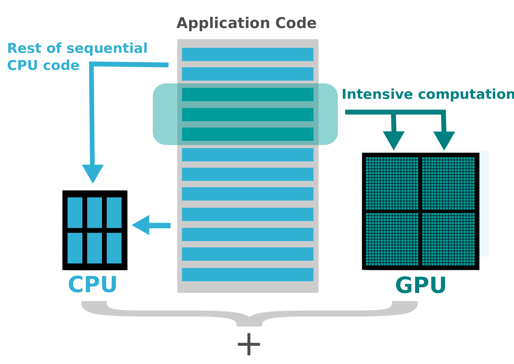
\includegraphics[scale=0.9]{img/gpgpu}
        \caption{Aceleración de programas en GPUs\cite{gpgpu}.}
        \label{fig:gpgpu}
    \end{figure}

    La unificación de los espacios de memoria facilita el GPGPU ya que no hay necesidad de transferencias explícitas de memoria entre el host y el dispositivo.


    %----------------------------------------------------------------------
    %SISTEMAS EMBEBIDOS
    \section{Sistemas embebidos}

    Un sistema embebido es un sistema de cómputo diseñado para realizar tareas dedicadas, donde el mayor retos es realizar tareas específicas donde la mayoría de ellas tengan requerimientos de tiempo real \cite{LimPree}.

    \subsection{Sistemas embebidos heterogéneos}
    %
    \vspace{0.3cm}
    En los últimos años los sistemas embebidos han ido demandando nuevas características debido a su rápida adopción en el mercado. Con lo que surge el desarrollo de sistemas embebidos heterogéneos, dónde está contemplado realizar una gran cantidad de cómputo pero con una gran eficiencia tanto energética como en espacio.
    \vspace{0.3cm}

    Actualmente la empresa NVIDIA tiene en su catálogo sistemas embebidos heterogéneos con un gran soporte y bibliotecas para el cómputo de alto rendimiento. Dichos sistemas cuentan con la arquitectura Pascal de última generación \cite{GPUArt}, la cual permite compartir memoria entre CPU y GPU.
   
    % Framework
    Debido a que la mayoría de las GPU en sistemas embebidos no son de naturaleza preemptive, es importante programar los recursos de GPU de manera eficiente en múltiples tareas \cite{TX2I} ya sea de planificación o memoria, lo que permite pensar en un framework que ayude a la administración de sus características. 

 \section{Material de trabajo}
 
Para realizar la presente tesis, se tuvo acceso al sistema embebido heterogéneo NVIDIA Jetson TX2, en el cual se realizaron algunas pruebas para la familiarización con esté tipo de dispositivos, así como la programación en tarjetas gráficas.

En la figura \ref{fig:arqutecturaTX2} se muestra diagrama de bloques de la arquitectura del sistema Jetson TX2.

      \begin{figure}[ht]
      \centering
        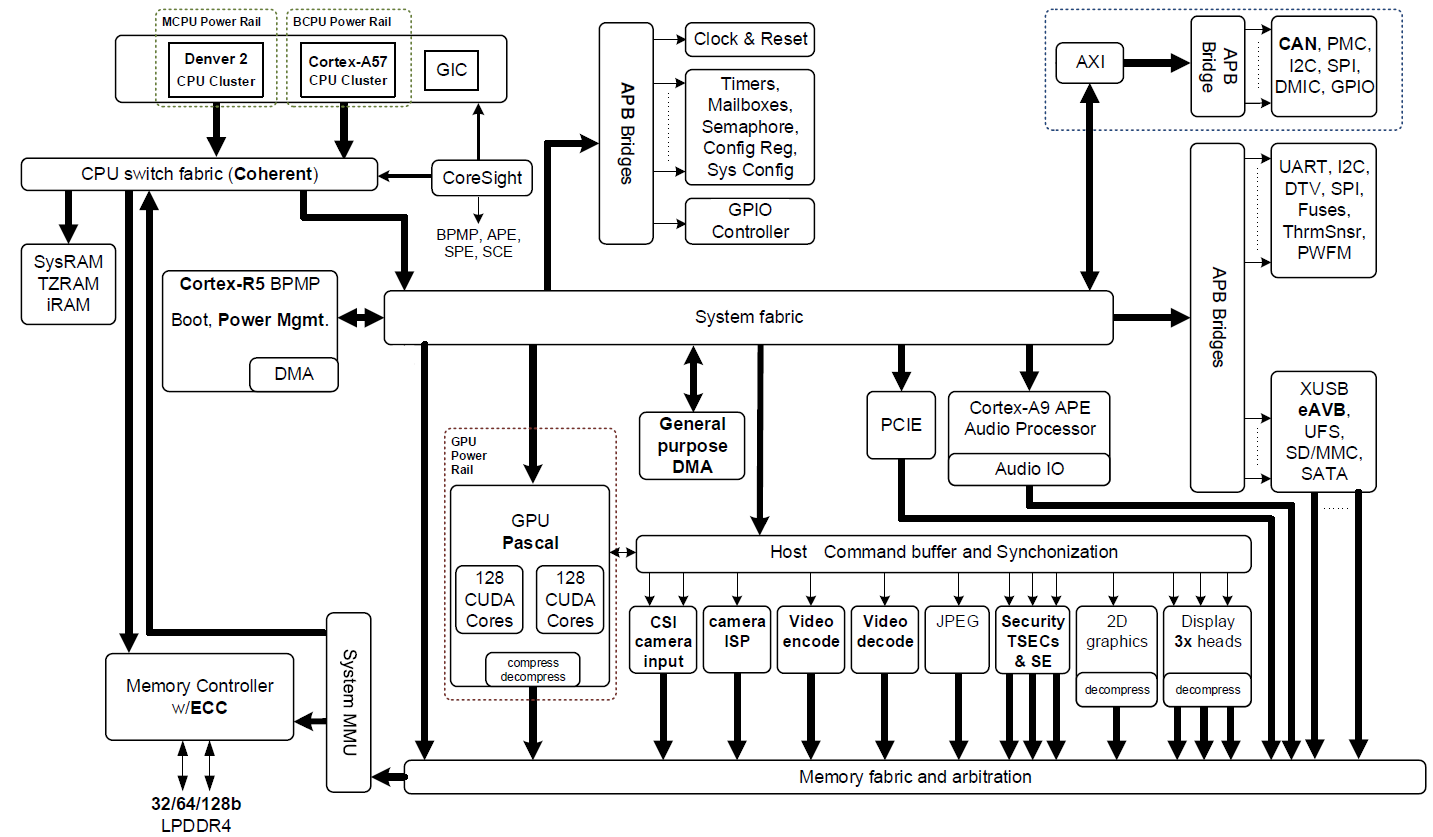
\includegraphics[scale=.45]{img/arqutecturaTX2}
        \caption{Diagrama de la arquitectura del sistema Jetson TX2\cite{ArqTX2}.}
        \label{fig:arqutecturaTX2}
    \end{figure}

 \subsection{Jetson TX2}
 
    Las especificaciones del sistema están descritas en la tabla \ref{tab:table1}.
    
    \begin{table}[h!]
      \begin{center}
            \scriptsize
        \begin{tabular}{|m{2.5cm}|m{6cm}|m{6.5cm}|}
         \hline
        \cellcolor{lightgray}\textbf{Elemento} & \cellcolor{lightgray} \textbf{Componentes} & \cellcolor{lightgray} \textbf{Descripción}\\ 
         \hline
         \textbf{Arquitectura} & NVIDIA Pascal GPU & 256 núcleos Optimizados para un mejor rendimiento en sistemas embebidos.\\
         \hline
         \textbf{CPU} & Dual-Core Denver 2 64-bit CPUs + Quad-Core A57 Complex & Contiene dos clústers de procesamiento, el Denver 2 de 64 bits que se utiliza para tareas pesadas o de un sólo thread; y el ARMv8 Cortex-A57 Complex que actúa en tareas multi-thread y en cargas ligeras.\\
         \hline
         \textbf{Memoria} & 8 GB L128 bit DDR4 Memory & DRAM de 128 bits que da soporte con un gran ancho de banda para una interfaz LPDDR4.  \\
          \hline
    	\textbf{Almacenamiento} & 32 GB eMMC 5.1 Flash Storage & Integrada en el módulo.\\
         \hline
    	\textbf{Conectividad} & 802.11ac Wi-Fi and Bluetooth-Enabled Devices & \\
         \hline
   	 \textbf{Ethernet} &10/100/1000 BASE-T Ethernet & \\
	  \hline
   	 \textbf{Procesador de señales} &1.4Gpix/s Advanced image signal processing & Acelerador por hardware para captura de video y de imágenes.\\
	 &Audio Processing Engine & Subsistema que permite el completo soporte de audio multicanal por las diversas interfaces.\\
	 \hline
   	 \textbf{Video} & Codificador avanzado de video HD & Permite la grabación de video ultra-high-definition a 60 fps, soporta los estándares H.265 and H.264 BP/MP/HP/MVC, VP9 y VP8. \\
	  & Decodificador avanzado de video HD & Reproducciónde video ultra-high-definition a 60 fps con pixeles de 12 bits, soporta los estándares H.265, H.264, VP9, VP8 VC-1, MPEG-2, y MPEG-4. \\
         \hline
   	 \textbf{Controlador de la pantalla} &eDP/DP/HDMI Multimodal & Realiza un almacenamiento multilínea de pixeles, lo que permite mayor eficiencia de memoria al momento de aplicar operaciones de escalamiento o de búsqueda de pixeles. Permite la reducción del ancho de banda en aplicaciones móviles.\\
         \hline
        \end{tabular}
        \caption{Especificaciones del sistema Jetson TX2\cite{jtx2dk}.}
        \label{tab:table1}
      \end{center}
    \end{table}
   
   Algunas de las tareas realizadas con el dispositivo incluyen desde la familiarización hasta la puesta a punto, como son:
   \begin{itemize}
    \item Instalación del Sistema Operativo Ubuntu 18 para procesadores ARM.
     \item Instalación de CUDA manager.
     \item Actualización de bibliotecas compatibles.
     \item Configuración de área local y conexión a travez de computadora remota.
      \item Investigación e implementación de ejercicios de GPGPU.
       \item Realización y modificación de ejercicios para la familiarización con la arquitectura Pascal, estructura de la tarjeta y su memoria.
    \end{itemize}   
   
    \section{Resumen}
\gls{maths}
Los CPU están diseñados para obtener el máximo rendimiento en un flujo de instrucciones ejecutando las tareas lo más rápido posible, pero un GPU está diseñado para procesar el mayor número de tareas tan rápido como sea posible en un tiempo reducido, por lo que se hace uso el cómputo paralelo en distintos dispositivos.

\subsection{Computación preemptive}
	La mayoría de los sistemas operativos modernos utilizan el cómputo preemption para planificar tareas, en una computadora que no utiliza tareas preemptive sólo se puede ejecutar un proceso a la vez con tofos los demás esperando en una cola hasta que se complete el proceso actual en ejecución. Por otra parte, una planificación de tareas preemptive elige un proceso y lo deja ejecutar durante un tiempo máximo llamado cuanto\cite{PreeK}, al llegar ese momento, se suspende y el planificador escoge otro dependiendo de las prioridades dadas o del algoritmo.

    %En este capítulo se presenta una breve introducción a la seguridad de la información, la importancia de incluirla en los sistemas de software y las amenazas a las que están expuestos los sistemas. Se hace un énfasis en la inclusión de la seguridad en la etapa de diseño de un sistema, donde se explica que utilizar guías para proporcionar un nivel de seguridad a un sistema en diseño disminuye las posibilidades de una amenaza al sistema ya implementado. 

    \subsection{Tipos de ejecución de tareas}

    Existen dos tipo de ejecución de tareas, las \textit{\textbf{preemptive}}, donde es necesario interrumpir temporalmente una tarea que está realizando un sistema de cómputo, para darle la oportunidad a otra con mayor prioridad, con el compromiso de reanudar la rezagada más adelante, y las \textit{\textbf{non-preemptive}} donde se requiere que termine la tarea actual para que posteriormente inicie una con mayor prioridad.

